\documentclass[12pt]{article}
    \usepackage{fullpage}
    \usepackage{fullpage}
    \usepackage{lipsum}
    \usepackage{filecontents}
    \usepackage[dvipsnames]{xcolor}
    \usepackage[english]{babel}
    \usepackage[utf8x]{inputenc}
    \usepackage{amsmath}
    \usepackage{amssymb}
    \usepackage{amsthm}
    \usepackage{graphicx}
    \usepackage[font=small,labelfont=bf]{caption}
    \usepackage[colorinlistoftodos]{todonotes}
    \usepackage{hyperref}
    \usepackage{cleveref}
    \usepackage[makeroom]{cancel}
    \usepackage{inconsolata}
    \usepackage{framed}
    \usepackage{algorithm}% http://ctan.org/pkg/algorithms
    \usepackage{algpseudocode}% http://ctan.org/pkg/algorithmicx
    \usepackage{mathtools}
    \usepackage{censor}
    \usepackage[dvipsnames]{xcolor}
    \usepackage{forloop}
    \usepackage{blkarray}
    \usepackage{makebox}
    \usepackage{subfig}

    
    \newcounter{ct}
    \newcommand{\markdent}[1]{\forloop{ct}{0}{\value{ct} < #1}
    {\hspace{\algorithmicindent}}}
    \newcommand{\markcomment}[1]{\Statex\markdent{#1}}

    \newcommand{\INDSTATE}[1][1]{\STATE\hspace{#1\algorithmicindent}}

    \captionsetup[algorithm]{labelformat=empty}
    \DeclareMathOperator{\EX}{\mathbb{E}}% expected value
    \DeclarePairedDelimiter\ceil{\lceil}{\rceil}
    \DeclarePairedDelimiter\floor{\lfloor}{\rfloor}
    
    \hypersetup{
    colorlinks,
    citecolor=Violet,
    linkcolor=Red,
    urlcolor=Blue}

    \hypersetup{
    citebordercolor=Violet,
    filebordercolor=Red,
    linkbordercolor=Blue
}
\begin{document}
%Header-Make sure you update this information!!!!
\noindent
\large\textbf{Classification of Electronic Music Subgenres Using CNNs}\\ 
 \\
\normalsize COMP4107 \hfill Alex Trostanovsky \\
Prof. White \hfill \\
TAs: Rui Li, Vasileios Lioutas \hfill Due Date: 16/12/18



\section*{Introduction}

The popularity of electronic dance music (EDM) has increased substantially in 
recent years 
\cite{c1}. In turn, EDM artists
adapt and experiment with 
different musical production elements associated with genres of
such as Techno, House, and Trance. In many cases, these
adaptations evolve to produce novel electronic music subgenres \cite{c2}\cite{c3}.\\
Outlined below is an investigation of the capacity of Convolutional Neural
Networks to classify the subgenres of a `niche' electronic
music genre: Psychadelic Trance. \\ We introduce relevant architectures 
which have been shown to correctly classify well-established musical 
genres such as: hip-hop, rock, and pop.\\
We experiment with various training hyperparameters and analyze their
impact on the classification accuracy of our model. Finally,
we discuss the results of our experiments, outline 
future research possibilities that may benefit from the results outlined 
in this report, and consider the application
of our model to music recommendation systems.\footnote{All code available
}

\section*{Background/related work}
Due to the recent shift in the music industry towards digital distribution,
automatic music recommendation systems have become a well 
researched and discussed
problem amongst online music providers such as 
\href{https://www.youtube.com/musicpremium}
{Youtube Music}, 
\href{https://www.apple.com/music/}
{Apple Music},and 
\href{https://www.spotify.com/}{Spotify}.\\
Recent implementations of Convolutional Neural Networks 
surpassed the genre classification accuracy metrics achieved  
by the use of traditional linear regression models.\cite{c4} \\ Using a CNN 
model that was trained on songs from the 
Million Song Dataset \cite{c5}, an AUC (area under the ROC, 
Reciever Operating Characteristic, curve: a plot of the True Positive
vs.
False Positive classification rate) of 0.77192 (with an upper bound of
0.96070) was achieved. \cite{c4}\\
The implementation of a CNN based genre classifier 
has since been adapted by 
Music Information Retrieval (MIR) 
researchers by incorporating Recurrent Components.\\
A CRNN (Convolutional Recurrent Neural Network) can be described
as a CNN in which the last convolutional layers are replaced
with a RNN (Recurrent Neural Network.)\\
CRNNs (Convolutional Recurrent Neural Networks) exhibited
strong performance with respect to the number of parameters 
and training time, achieving a consistently higher
AUC-ROC ($\ge 0.85$), when compared to traditional CNNs.\cite{c6}

\subsubsection*{Possible Bias in Training Data}
Upon review of the relevant work, we noted that most of the 
research that has demonstrated the effectiveness of CNNs/CRNNs 
in the domain of automatic music genre
classification focused on the same datasets (Million Song Dataset, 
Free Music Archive (FMA))\cite{c7}. 
In addition, the models that were trained
on these datasets mainly considered only the `top 50' tags (`rock',
`hip-hop', `pop').\\
Such genres possess
discriminating musical features that could aid in their classification.\\
For example, the dominant use of electric guitars in `rock' music, 
or the use of `Drum Machines' (electronical musical instruments
that imitate percussive sounds) in `hip hop'. Such features are 
usually indicative 
of songs belonging to these genres.
\section*{Problem Statement}
Can CNNs achieve the same strong classification metrics when trained
on `niche' Electronic Music subgenres that posses a lower degree 
of genre discernability when compared to popular music genres
such as `rock' and `hip hop'?

\section*{Data Preparation}
To answer our problem statement, we required a (relatively) large dataset of 
songs that were established exemplars of 
Psychadelic Trance subgenres.\\
Psychadelic Trance is, itself, a subgenre of trance music that is characterized
by rhythm arrangements overlaid with high tempo melodies 
and basslines. \\
A collection of 920 Psy-trance tracks were obtained from 
\href{http://www.ektoplazm.com/}{Ektoplazm}, a  
source of `free and legal psytrance, techno and downtempo music' that
has served more than 21 million Creative Commons-licensed releases.\\
The 920 tracks that make up the dataset consist of:
\begin{itemize}
    \item 184 Dark-Psytrance tracks - 
    BPM (Beats Per Minute) range: $\ge 148$
    \item 184 Downtempo tracks  - Ambient, with Avg. BPM range: $\le 120$
    \item 184 Full-on tracks -  Avg. BPM range: $\approx 145$
    \item 184 Goa Tracks - Melodic, with BPM range: $\approx 145$
    \item 184 Techno tracks - BPM range: $\le 130$
\end{itemize}
All genre labels were obtained from HTML tags present in the repository.\\
Since Trance music is heavily reliant on a repetitive 4/4 time signature, 
some of the chosen subgenres (Full-on, Goa, Dark) may sound very similar 
due to their similar use of instrumentation. For example, 
different training examples may utilize the same synthesizers
to produce basslines and kick drums 
that take up equivalent frequency ranges.\\
In addition, the datset includes compositionally distinct subgenres such 
as Techno and Downtempo.
\subsection*{Preprocessing}
Each track was processed using the core IO functionalities included
in the music and audio analysis python package 
\href{http://librosa.github.io/librosa/}{\tt libROSA}\cite{c8}.\\
All tracks were sampled at 44100 Hz (Mono) and a 
Log-amplitude mel-spectrogram
was computed for each track.\\ 
The mel scale is a quasi-logarithmic function of acoustic frequency.
A mel scale spectrogram 
groups together perceptually similar 
pitch intervals (such as octaves) into `bins' so that
they appear equal in width over the full hearing range \cite{c9}.\\
CNN models that were trained on Mel-Frequency spectrograms
have been shown to achieve a higher degree
of classification accuracy when compared to other forms of audio
representation \cite{c6}.\\
Each track was further segmented into slices of 128 pixels $\times$
128 mel-frequency bins (essentially a visual representation 
of a 2.56s window in a track).\\
To construct the training and testing dataset, the midpoint of 
each track was calculated and 30 spectrograms slices were extracted
from around that midpoint.
\begin{center}
    \makebox[\textwidth]
    {
        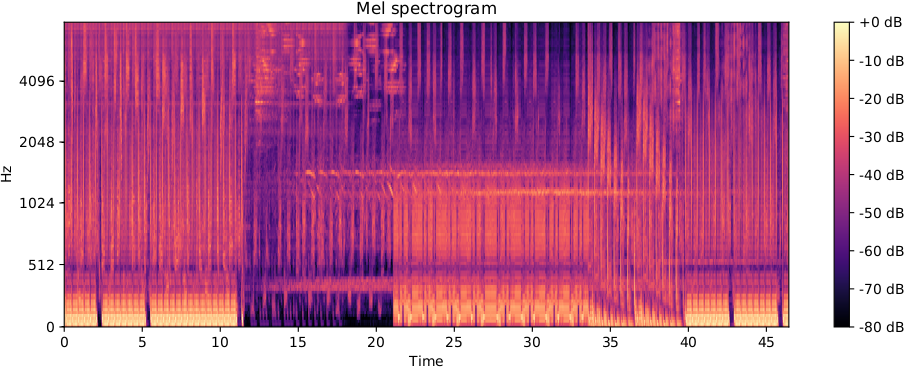
\includegraphics[scale=0.4]{./diagrams/dark_spec_01.png}
    }
    \captionof{figure}{A Log-amplitude Mel-Spectrogram}
\end{center}


\section*{Model}
The architecture was based on a CNN model which has been 
shown to achieve a high classification accuracy when trained on 
mel-spectrograms of audio tracks\cite{c4}.\\ Implementational details
were adapted from a finalist solution to the 
\href{https://www.crowdai.org/challenges/www-2018-challenge-learning-to-recognize-musical-genre}
{CrowdAI WWW Musical Genre Recongition Challenge}. 

\begin{center}
    \makebox[\textwidth]
    {
        \includegraphics[scale=0.27]{./diagrams/1_cnn.pdf}
    }
    \captionof{figure}{A sample CNN architecture. The time axis 
    (which is convolved over) is vertical.}
\end{center}
As opposed to traditional square convolutional filters, 
the filter that was chosen across layers was rectangular. 
The convolutions are one dimensional, and happen only across
the time dimension, and not in the mel-frequency dimension.\\
Using square filters is appropriate in cases where
the two axes of an image represent the same feature (pixels $\times$ pixels),
whereas the axes of mel-spectrograms represent time and frequency.\\
After the last convolutional layer, a global temporal pooling layer
was introduced. This layer pools across the entire time 
axis, and computes aggregate statistics (Mean, Max) of the learned 
features across time \cite{c4}.

\subsection*{Training}
30 spectrogram slices were extracted from each track to create a dataset
of $920\times30=27600$ samples.\\
Training was performed in 5-folds. For each fold, 
the model was trained on 22080 samples, and tested 
on 5520 samples. \\
We ensured that for each data batch consumed during training and 
testing, an equal distribution of all 5 subgenre classes 
was maintained.
This was done by creating protocol buffered,
\href{https://www.tensorflow.org/tutorials/load_data/tf-records}
{\tt TFRecord} files that contained a permuted array of 
150 spectrogram slices (30 per subgenre). 

\section*{Experiments}

Three experiments were conducted to investigate the performance
of the model using different configurations 
of hyperparameters. All experiments were performed in an Ubuntu 18.04.1 LTS
Linux Environment, on an Intel(R) Core(TM) i5-4690K CPU. \\
Model compilation, training, testing, and predictions were evaluated in 
a \href{https://keras.io/}{\tt Keras}, GPU-enabled, 
\href{https://github.com/keras-team/keras/tree/master/docker}{\tt Docker} 
image, using a GeForce GTX 1070Ti GPU. 

\subsection*{Experiment 1: Dropout Probabilities}
Models trained using Dropout have been shown to develop more robust 
feature representations \cite{c13}. When training, a certain amount of neurons in 
the network (proportional to the dropout {\tt keep\_prob} parameter)
is randomly removed. 
This causes the activated neurons to `rely' less on their neighbours, 
and generate non-zero gradients.
\\ Using Dropout can be viewed as sampling
from an exponential weight configuration search space. 
When a certain weight configuration performs optimally, 
it will reinforce the neurons
and weights which made up that configuration.\\
While the base model (from which our model was adapted) utilized a 
dropout probability of 0.2, we were interested to investigate the performance
of higher dropout probabilities.

\subsection*{Experiment 2: Optimizers}
The following optimizers were asssesed \cite{c11} :
\begin{itemize}
    \item {\tt Adadelta:}\\
    Adapts learning rates based on a moving window of gradient updates,
    instead of accumulating all past gradients.
    \item {\tt Adam:}
    Calculates a moving average of the gradient and the 
    squared gradient, and uses hyperparameters to maintain decay rates
    of these moving averages.
    \item {\tt Adamax:}\\
    A generalization to the $L^2$ norm based update rule of {\tt Adam}
    using the $L^\infty$ norm. \cite{c12}
    \item {\tt SGD:} (Stochastic Gradient Descent)\\
    Random samples from the dataset allow timely estimation of 
    gradients in a large search space.
\end{itemize}
\subsection*{Experiment 3: Global Pooling Layer}
The addition of a global temporal pooling layer following 
the convolutional layers is due to the nature of the task of genre 
classification. \cite{c10}\\
In general, CNNs use the absolute location 
of features to classify images. For example, a circular shape could either mean 
a wheel or a frisbee, depending on the location of the shape in the 
image. \\However, a correct classification of the genre of a spectrogram slice  
does not depend on an optimal detection of the \textit{locations} 
of latent features. Instead, the overall absence or presence of features
can inform correct classifications of genres. 
For example, the presence of 
a repetitive kick drum pattern may be indicative of a Full-on track,
while a smooth spectrogram across slices will likely represent 
a downtempo/ambient track.\\
Therefore, we investigated classification accuracy with the original 
global temporal pooling layer (a concatenated {\tt MAX + MEAN pool}),
or with either a {\tt MAX pool} or {\tt MEAN pool} global temporal layer. 

\section*{Results}
\begin{figure}[H]%
    \centering
    \subfloat{{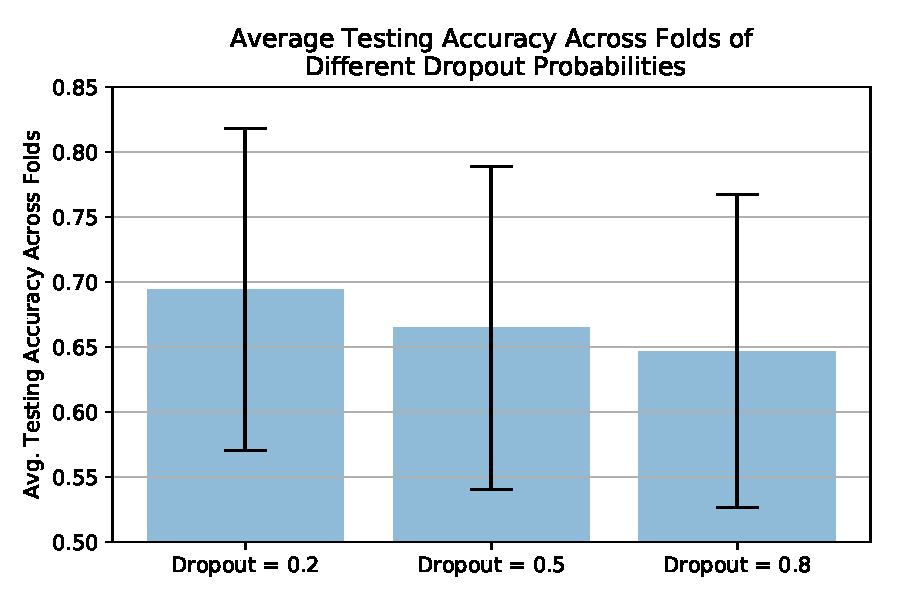
\includegraphics[scale=0.50]
    {./diagrams/dropout_bar.pdf} }}%
    \qquad
    \subfloat{{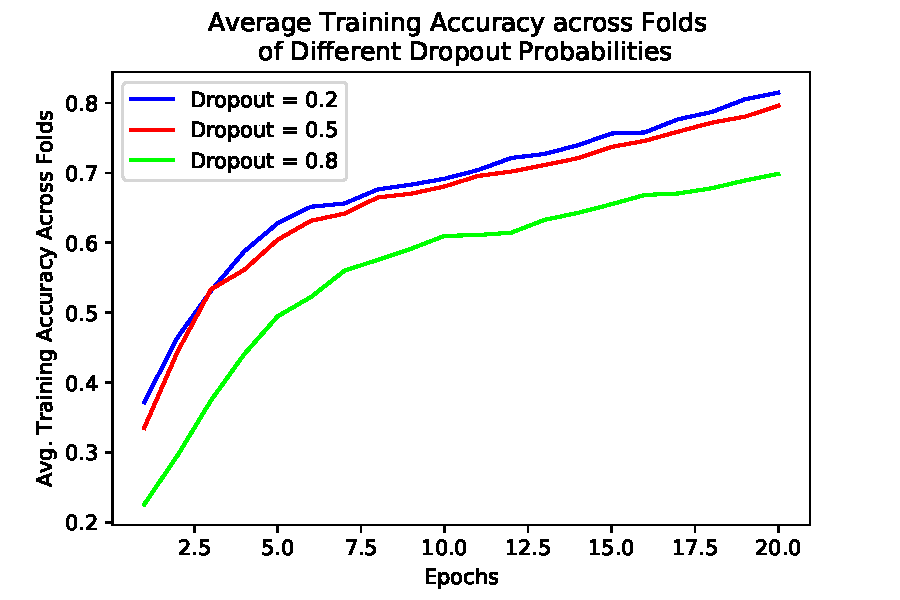
\includegraphics[scale=0.50]
    {./diagrams/dropout_lines.pdf} }}%
    \caption{
        Experiment 1: Dropout. All models trained with 
        {\tt Adam}, {\tt MAX+MEAN} pooling layer.            
        }       
    \label{fig:example}%
% \end{figure}
% \begin{figure}[H]%
    \centering
    \subfloat{{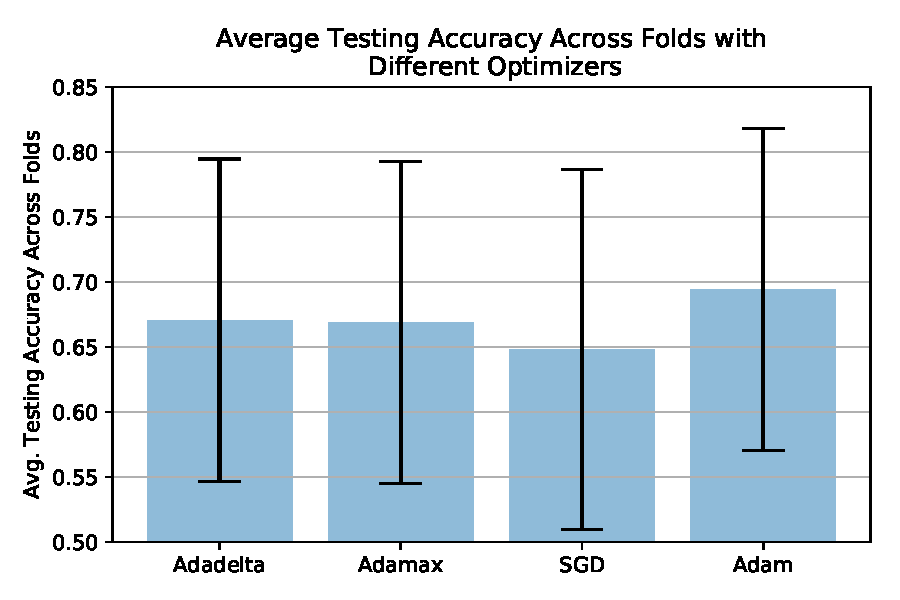
\includegraphics[scale=0.50]
    {./diagrams/opt_bar} }}%
    \qquad
    \subfloat{{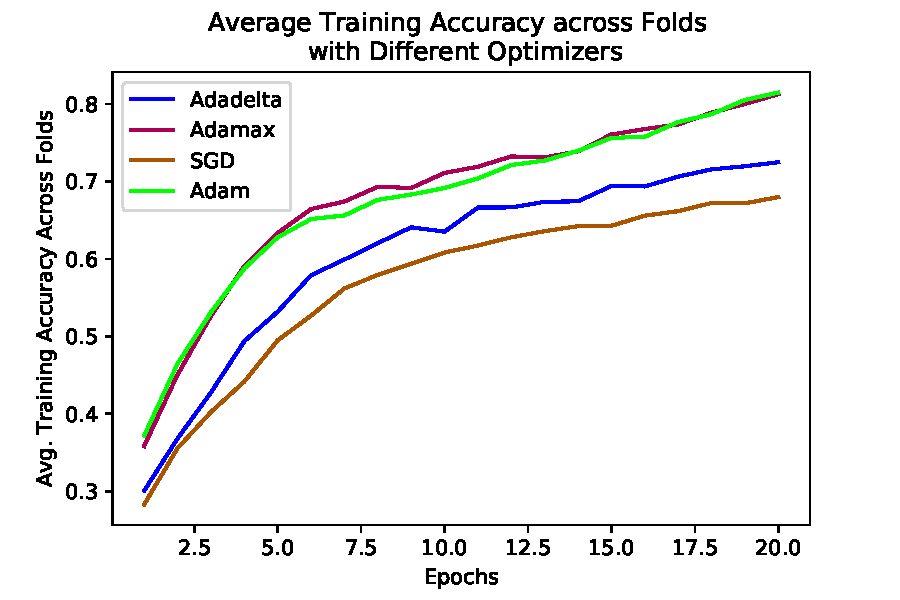
\includegraphics[scale=0.50]
    {./diagrams/opt_lines} }}%
    \caption{Experiment 2: Optimizers. 
    All optimizers trained 
    with {\tt keep\_prob} = 0.2}%
    \label{fig:example}%
% \end{figure}
% \begin{figure}[H]%
    \centering
    \subfloat{{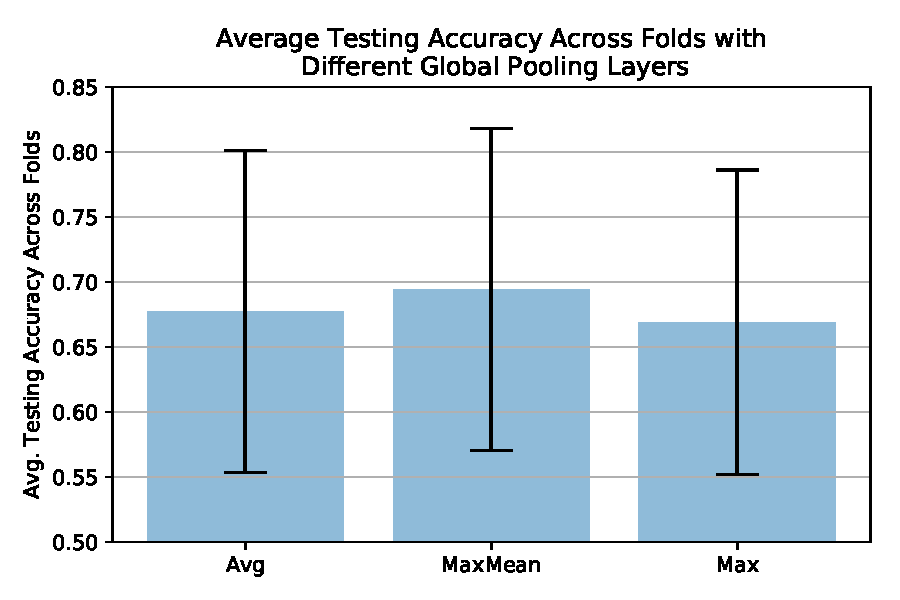
\includegraphics[scale=0.50]
    {./diagrams/pool_bar} }}%
    \qquad
    \subfloat{{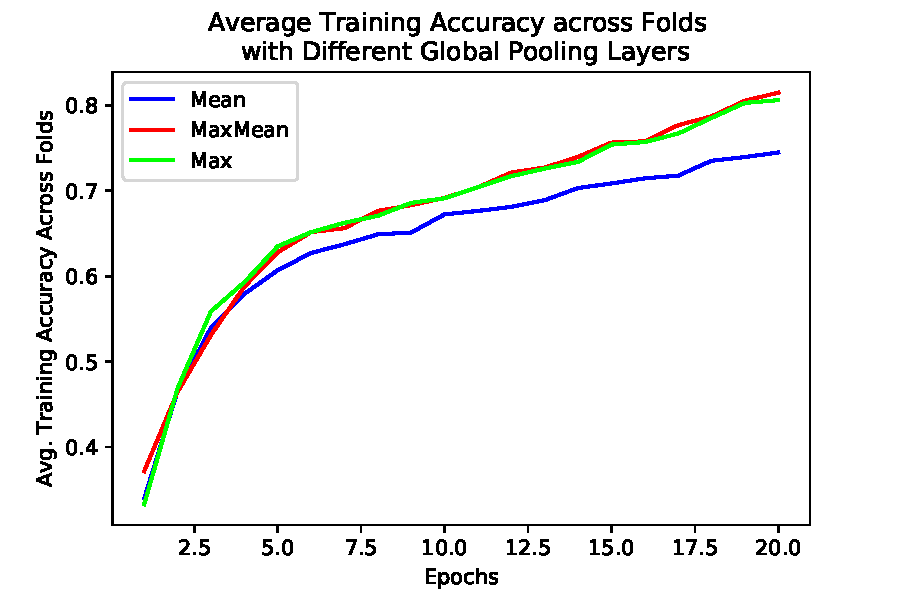
\includegraphics[scale=0.50]
    {./diagrams/pool_lines} }}%
    \caption{Experiment 3: Global Pooling. All models 
    trained 
    with {\tt keep\_prob} = 0.2 and {\tt Adam}}%
    \label{fig:example}%
\end{figure}

\section*{Analysis}

We conclude that the hyperparameter configuration 
(Dropout probability = 0.2, {\tt Adam} Optimizer, with a 
{\tt Max+Mean} global temporal pooling layer)
chosen by the original authors of the architecture was optimal.
Note that in all three experiments, accuracy on the training
data is closely matched by other possible configurations (Dropout = 0.5
in experiment 1, {\tt Adamax} in experiment 2, and just 
a {\tt Max} pooling layer in experiment 3). However, if performance
on the unseen testing set is also considered, 
then the original hyperparameter
configuration performed optimally
in both training and testing.\\
Classification on the testing set did not achieve an
accuracy $\ge 70\%$. We believe this was due to the manner
in which data was presented for testing. When testing the model, 
batches of 150 randomly ordered spectrogram slices 
(30 of each genre) were presented.
To calculate the accuracy of the model, the number of correct 
classifications were divided by the total training samples in the batch.\\
We decided to re-evaluate the prediction performance of our model 
in the following manner: instead of shuffling
150 samples of 5 different tracks, we presented the model 
with 30 spectrograms from the midpoints of a selection of novel tracks
(unseen in both training and testing)
belonging to the 5 classes. The model computed the predictions
for each of the 30 spectrograms. To classify a track, the 
dominant classification out of the 30 would be chosen. For example, 
if presented with a Full-on track, we would expect some of the 
spectrograms to be classified as either Goa, or Dark, since they 
occupy a similar BPM and frequency range. However, if the majority
of the spectrograms were classified as `Full-on', 
the prediction would be considered accurate.\\
After training a model using the optimal hyperparameter configuration,
the model achieved 
an $84\%$ correct prediction rate when presented with
51 novel tracks (with approximately 10 tracks per class).
\section*{Discussion}
As was anticipated, most misclassifications occurred between tracks
belonging to
genres with a similar BPM or Instrumentation Frequency Range 
(Goa, Dark, Full-on). \\Surprisingly, a substantial amount of 
the misclassifications occurred when the model 
incorrectly predicted a track
was Downtempo. We hypothesize that these tracks were misclassified 
because the 30 spectrograms (that were
extracted from the midpoint of the track) 
did not contain representative features which were associated 
with the track's genre. This can happen if the spectrograms 
for a track were contained in a segment of the 
track known as a Breakdown or a Drop (sudden changes in 
rhythm or bass line).
\begin{figure}[H]%
    \centering
    \subfloat[Correctly classified as `Goa']{{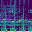
\includegraphics[scale=7]
    {./diagrams/correct_goa.pdf} }}%
    \qquad\hspace{15mm}
    \subfloat[Misclassified as `Downtempo']{{
\includegraphics[scale=7]
    {./diagrams/incorrect_goa.pdf} }}%
    \caption{
        Two slices of two different Goa tracks. (a) was correctly 
        classified as it exhibits the common 4/4 kick pattern, while 
        (b) likely represents a break/drop, and so was misclassified.           
        }       
    \label{fig:example}%
\end{figure}

To address this, an alternative spectrogram segmentation strategy may 
be used.\\ Instead of arbitrarily choosing the midpoint of a track as the 
representative locus around which spectrograms are extracted,
one could use onset detectors \cite{c14}, or beat and tempo trackers 
\cite{c15}, to 
preprocess an audio track. Using these results, the choices of loci
around which one segments an audio track may be more informed,
and provide more relevant data with which to train CNN models.\\
Finally, as was mentioned earlier, future research may also 
investigate the accuracy performace of CRNNs in genre classification
of Electronic Music. Since RNNs have been shown to be flexible 
in the summarization of local features \cite{c6}, issues 
of misclassifications due to unrepresentative segmentations (as were
shown by our preprocessing of the data) may be resolved by: a) making
informed choice about samplings locations within an audio track and b)
using a Recurrent Architecture that takes into account the global
structure of an audio track.
\section*{Conclusions}
We have shown that CNNs trained on 
Log-amplitude mel-spectrograms  
of Psychadelic Trance audio tracks can achieve a 84\% correct subgenre 
classification
metric when presented with novel samples. Previous research has
shown that CNN/CRNNs perform strongly in the domain of genre classification
of popular music. The results obtained in this report indicate that 
strong automatic
music genre classification by CNNs is not necessarily genre dependant. 
\\\\
The increasing popularity of electronic music, along with the growing demand
for online music recommendation services, 
should be considered when developing intelligent 
recommendation systems that can correctly identify 
new trends in Electronic Music. It appears that CNNs can learn 
the latent features that set trending subgenres apart, but to do so, 
models should be trained on 
modern datasets that contain examples of the current Electronic Music 
landscape.
% trending genres to learn the differentiating factors and latent 
% features that set subgenres apart.
\clearpage
\begin{thebibliography}{99}
\bibitem{c1}
{
    
    It's a \$6.2 billion industry. But how did 
    Electronic Dance Music get so popular?. (2015, October 30). CNN. 
    Retrieved from 
    \href {https://www.cnn.com/2014/12/18/world/how-did-edm-get-so-popular/index.html}
    {https://www.cnn.com/2014/12/18/world/how-did-edm-get-so-popular/index.html}
}
\bibitem{c2}
{   
    Timeline of electronic music genres.
    In Wikipedia. Retrieved December 15, 2018
    \href{https://en.wikipedia.org/wiki/Timeline_of_electronic_music_genres}
    {https://en.wikipedia.org/wiki/Timeline\_of\_electronic\_music\_genres}
}
\bibitem{c3}
{
    McLeod, K. (2001).
    Genres, subgenres, sub-subgenres and more:
    Musical and social differentiation within electronic/dance 
    music communities. 
    \textit{Journal of Popular Music Studies}, 13(1), 59-75.
}
\bibitem{c4}
{
    Van den Oord, A., Dieleman, S., \& Schrauwen, B. (2013). 
    Deep content-based music recommendation. 
    In \textit{Advances in Neural Information Processing Systems} 
    (pp. 2643-2651).
}
\bibitem{c5}
{
    Thierry Bertin-Mahieux, Daniel P.W. Ellis, Brian Whitman, and Paul Lamere. 
    The Million Song Dataset. In Proceedings of the 12th \textit
    {International Society
    for Music Information Retrieval Conference} (ISMIR 2011), 2011.

}
\bibitem{c6}
{
    Choi, K., Fazekas, G., Sandler, M., \& Cho, K. (2017, March). 
    Convolutional recurrent neural networks for music classification. 
    In \textit{2017 IEEE International Conference on Acoustics, Speech 
    and Signal 
    Processing (ICASSP)} (pp. 2392-2396). IEEE.
}
\bibitem{c7}
{
  
  Defferrard, M., Benzi, K., Vandergheynst, P., \& Bresson, Xavier.
  FMA: A Dataset for Music Analysis.
  \textit{18th International Society for Music Information 
  Retrieval Conference}.
  2017
  \href{https://github.com/mdeff/fma}
  {https://github.com/mdeff/fma}
}

\bibitem{c8}
{
    Brian McFee, Matt McVicar, Stefan Balke, Carl Thomé, 
    Vincent Lostanlen, Colin Raffel, ... Adrian Holovaty. 
    (2018, August 9). librosa/librosa: 0.6.2 (Version 0.6.2). 
    Zenodo. 
    \href{http://doi.org/10.5281/zenodo.1342708}
    {http://doi.org/10.5281/zenodo.1342708}
    
}
\bibitem{c9}
{
    \href{https://librosa.github.io/librosa/generated/librosa.core.mel_frequencies.html}
    {https://librosa.github.io/librosa/generated/librosa.core.mel\_frequencies.html}
}
\bibitem{c10}
{
    Dieleman, S. (2014). 
    \textit{Recommending music on Spotify with deep learning.} 
    Sander Dieleman, 5.
    Retrieved from 
    \href{http://benanne.github.io/2014/08/05/spotify-cnns.html}
    {http://benanne.github.io/2014/08/05/spotify-cnns.html}
}
\bibitem{c11}
{
\href{https://keras.io/optimizers/}
{https://keras.io/optimizers/}
}
\bibitem{c12}
{
    Kingma, D. P., \& Ba, J. (2014). 
    Adam: A method for stochastic optimization. 
    \textit{arXiv preprint arXiv:1412.6980.}
}
\bibitem{c13}
{
    Srivastava, N., Hinton, G., Krizhevsky, A., 
    Sutskever, I., \& Salakhutdinov, R. (2014). 
    Dropout: a simple way to prevent neural networks from overfitting. 
    \textit{The Journal of Machine Learning Research}, 15(1), 1929-1958.
}
\bibitem{c14}
{
    \href{https://librosa.github.io/librosa/onset.html}
    {https://librosa.github.io/librosa/onset.html}
}
\bibitem{c15}
{
    \href{https://librosa.github.io/librosa/beat.html}
    {https://librosa.github.io/librosa/beat.html}
}
\end{thebibliography}

\end{document}